\documentclass[11pt]{article}
\usepackage[utf8]{inputenc}
\usepackage[dvips]{graphicx}
\usepackage{fancybox}
\usepackage{verbatim}
\usepackage{array}
\usepackage{latexsym}
\usepackage{alltt}
\usepackage{hyperref}
\usepackage{textcomp}
\usepackage{color}
\usepackage{amsmath}
\usepackage{amsfonts}
\usepackage{rotating}
\usepackage{tikz}
%\usepackage{fitch}  % to use fitch
\usepackage{float}
\usepackage[hmargin=3cm,vmargin=5.0cm]{geometry}
\usepackage{graphicx}
\graphicspath{ {./} }
%\topmargin=0cm
\topmargin=-2cm
\addtolength{\textheight}{6.5cm}
\addtolength{\textwidth}{2.0cm}
%\setlength{\leftmargin}{-5cm}
\setlength{\oddsidemargin}{0.0cm}
\setlength{\evensidemargin}{0.0cm}

\begin{document}
	\section*{Student Information } 
	%Write your full name and id number between the colon and newline
	%Put one empty space character after colon and before newline
	Full Name :  Ahmet Eren {\c C}olak \newline
	Id Number :  2587921 

	\section*{Q. 1}
	Only 1 query is sent to a DNS server for retrieving the \emph{ceng.metu.edu.tr}'s IP address.
	
	\begin{center}
		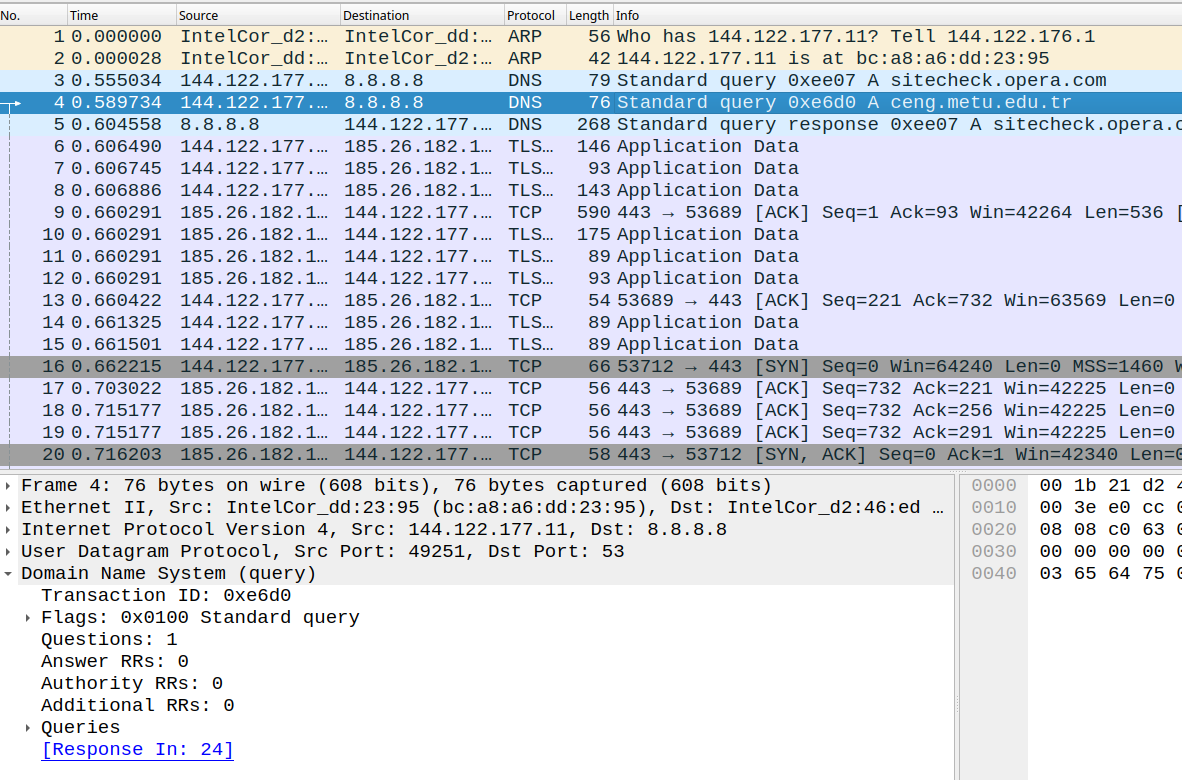
\includegraphics[scale=0.25]{dnsquery}
	\end{center}

	\section*{Q. 2}
	Only 1 server is queried for the DNS request.
	
	\section*{Q. 3}
	IP address of the queried DNS server is 8.8.8.8
	
	\section*{Q. 4}
	It is not possible to tell whether the response is cached or not.
	If there were multiple DNS requests, then it would be possible to tell whether it is cached by comparing TTL times of responses.
	\section*{Q. 5}
	
	\begin{center}
		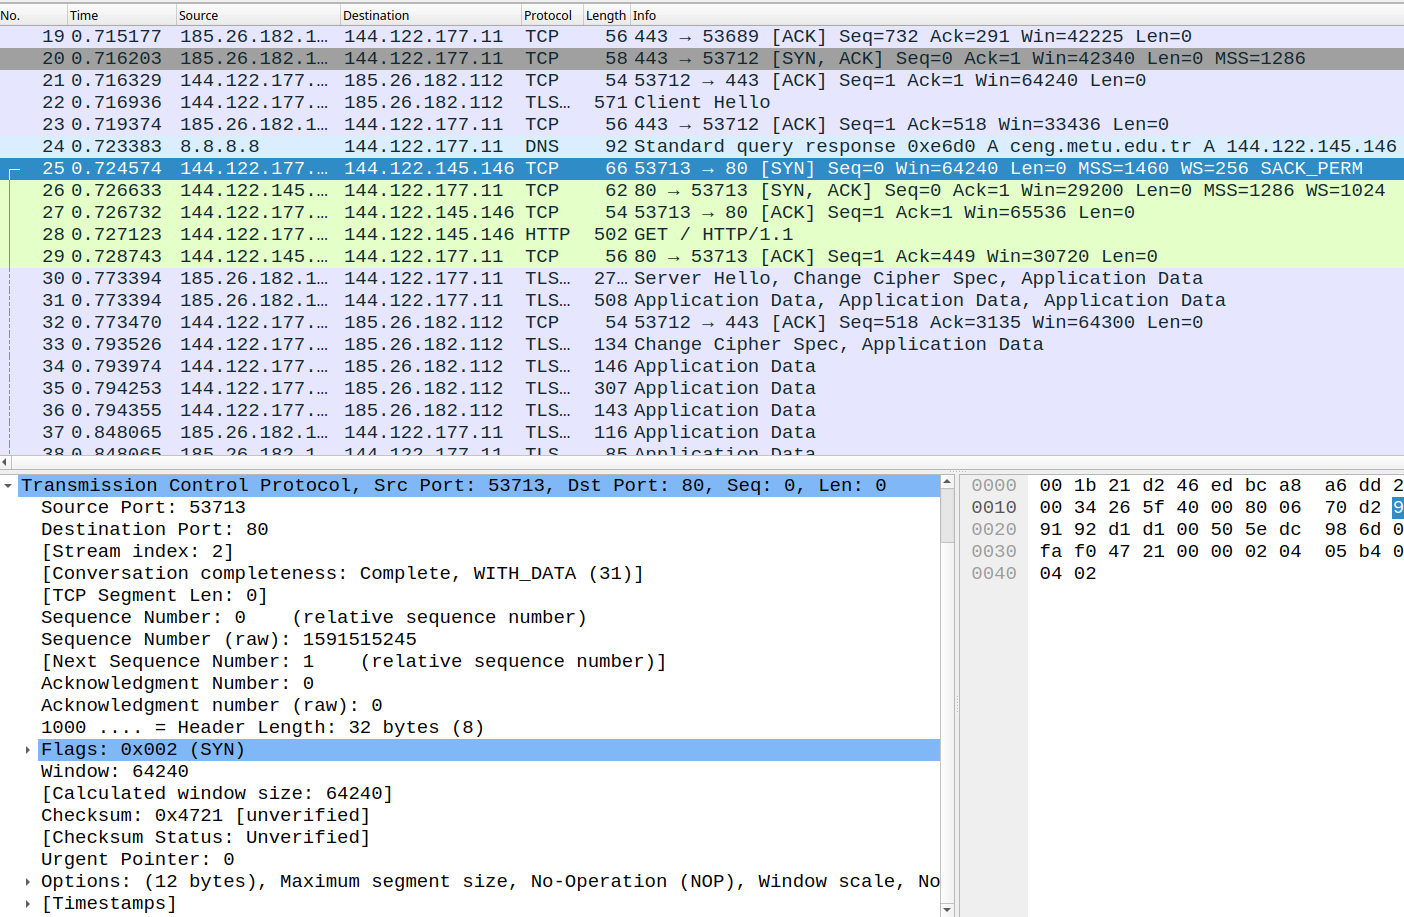
\includegraphics[scale=0.25]{tcppair}
		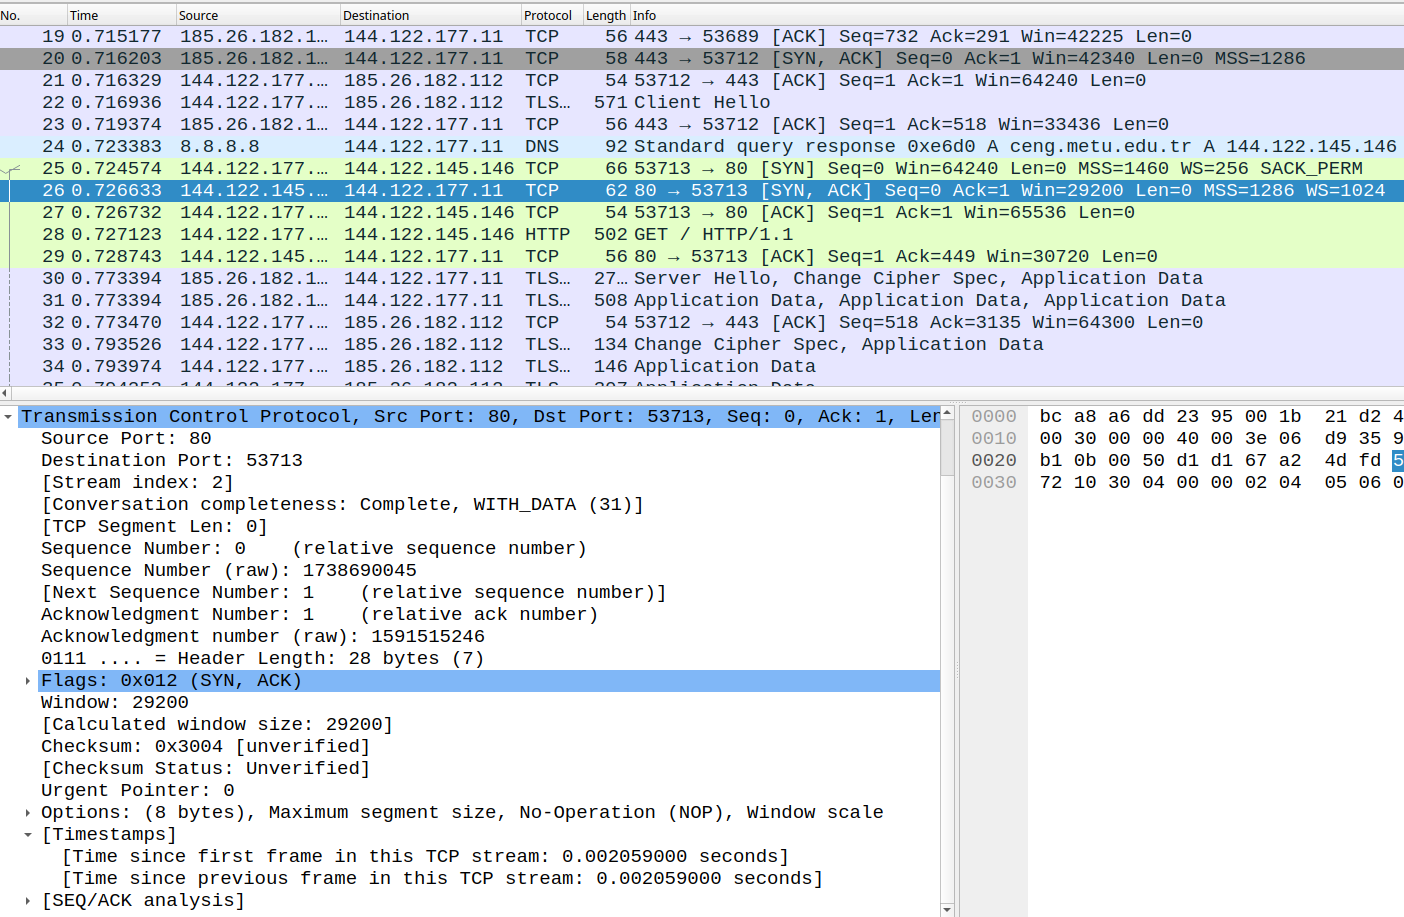
\includegraphics[scale=0.25]{tcppair2}
	\end{center}
	
	\subsection*{a.}
	Protocol of these requests is TCP.
	\subsection*{b.}
	HTTP is relies on TCP. Thus, a TCP connection must be established before exchanging HTTP messages. Because of that the protocol used in first request and response pair is TCP.
	\subsection*{c.}
	It is 0.002059 seconds.
	
	\section*{Q. 6}
	No, there is not any cookies sent with the first HTTP request.
	\begin{center}
		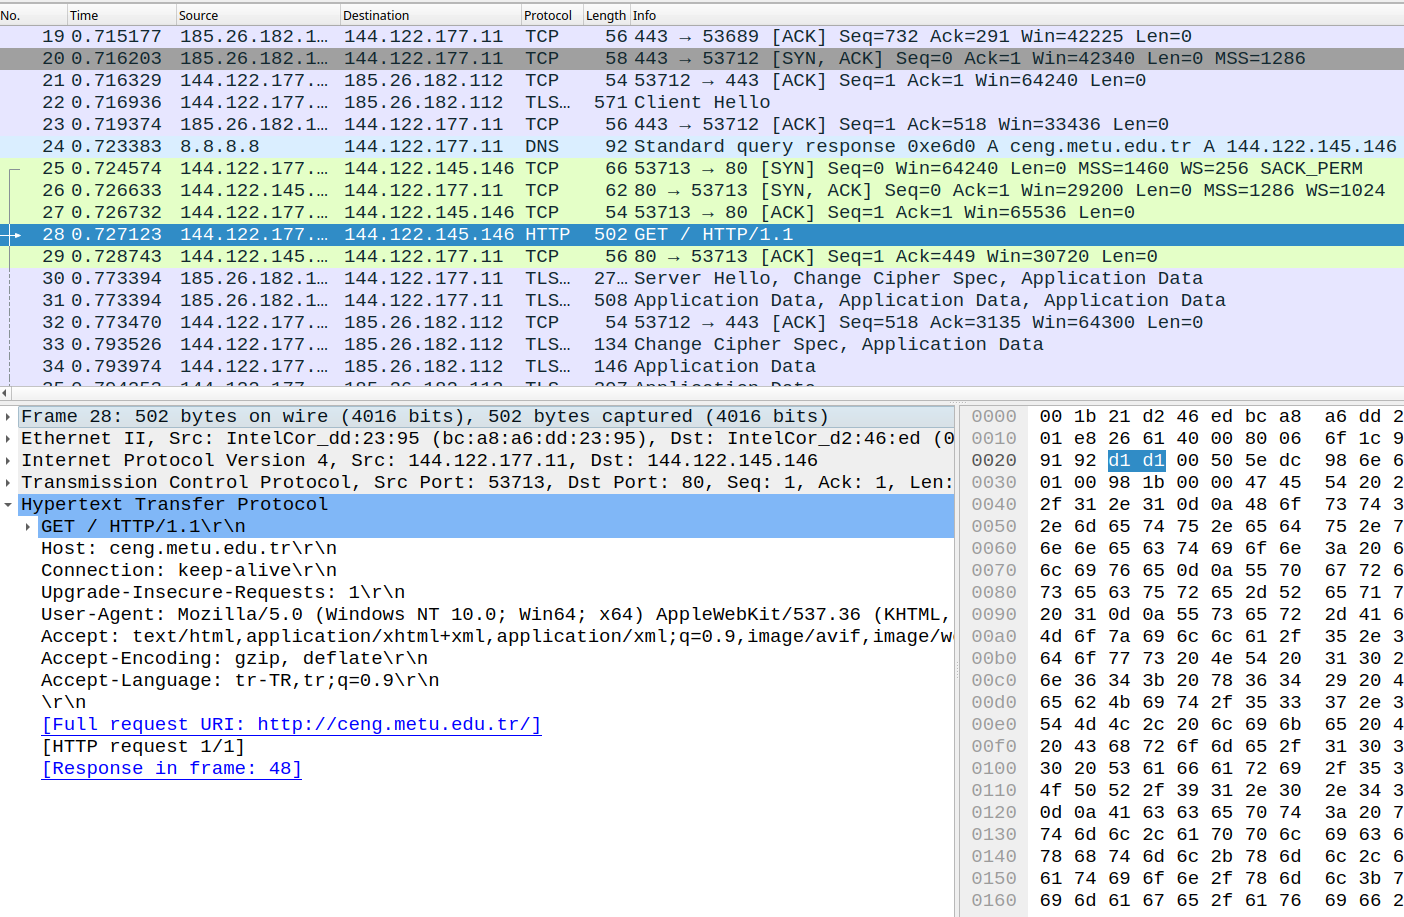
\includegraphics[scale=0.25]{firsthttp}
	\end{center}
	\section*{Q. 7}
	\subsection*{a.}
	It is: "User-Agent: Mozilla/5.0 (Windows NT 10.0; Win64; x64) AppleWebKit/537.36 (KHTML, like Gecko) Chrome/105.0.0.0 Safari/537.36 OPR/91.0.4516.77"
	\subsection*{b.}
	User-agent string include the browser I used which was Opera. It can be seen at the end of the string ("OPR/91.0.4516.77"). It also mentions about Safari and Chrome. This is probably because Opera wants web servers to identify itself as Chrome or Safari as well.

	\section*{DNS}
	It is not possible to send an email to \emph{merkel@de}. Because domain name of the email server ("de") lacks a top level domain. Therefore DNS servers will not be able to resolve it. 
\end{document}